\documentclass{beamer}
\usepackage[utf8]{inputenc}
\usepackage{listings}
\usepackage{color}
%\usetheme{Singapore}
\title[Ideal Library]{Ideal Library}
\author{Rafael Fernández López}
\institute{http://www.ereslibre.es/projects/ideal\\ereslibre@kde.org}
\date{}

\pdfinfo
{
  /Title       (IDEALLIBRARY)
  /Creator     (KILE)
  /Author      (RAFAEL FERNANDEZ LOPEZ)
}

\definecolor{gray97}{gray}{.97}
\definecolor{gray75}{gray}{.75}
\definecolor{gray45}{gray}{.45}

\lstset{ frame=Ltb,
         framerule=0pt,
         aboveskip=0.5cm,
         framextopmargin=3pt,
         framexbottommargin=3pt,
         framexleftmargin=0.4cm,
         framesep=0pt,
         rulesep=.4pt,
         backgroundcolor=\color{gray97},
         rulesepcolor=\color{black},
         %
         stringstyle=\ttfamily,
         showstringspaces = false,
         basicstyle=\scriptsize\ttfamily,
         commentstyle=\color{gray45},
         keywordstyle=\bfseries,
         %
         numbers=left,
         numbersep=-5pt,
         numberstyle=\tiny,
         numberfirstline = false,
         breaklines=true
      }

\setbeamertemplate{navigation symbols}{}

\begin{document}

\begin{frame}
  \titlepage
\end{frame}

\section*{}
\begin{frame}{}
  \framesubtitle{}
  \tableofcontents[section=1]
\end{frame}

\newcommand<>{\highlighton}[1]{%
  \alt#2{\structure{#1}}{{#1}}
}

\newcommand{\icon}[1]{\pgfimage[height=1em]{#1}}

\section{¿Qué es?}

\begin{frame}{¿Qué es?}
  Ideal Library es un conjunto de librerías que permiten desarrollar
  aplicaciones de una manera sencilla e intuitiva.\\
  \bigskip
  API similar a Qt en ciertos aspectos.
  \bigskip
  \begin{itemize}
    \item Sencilla
    \medskip
    \item Consistente
    \medskip
    \item Correcta
  \end{itemize}
\end{frame}

\section{Ventajas}

\begin{frame}{Ventajas (1 de 2)}
  \begin{itemize}
    \item No existe concepto de slot
      \begin{itemize}
        \item Todos los métodos (ya sean estáticos, miembro o funciones estáticas)
          pueden ser destino de una conexión
      \end{itemize}
    \pause
    \medskip
    \item Corrección de las conexiones comprobada en tiempo de compilación
    \pause
    \medskip
    \item Señales y slots respetan el ámbito en el que son declarados
  \end{itemize}
\end{frame}

\begin{frame}{Ventajas (2 de 2)}
  \begin{itemize}
    \item Es conocido el orden en que un disparo de una señal llamará a los slots/señales
    \pause
    \medskip
    \item Si cambia la firma de alguna señal o slot no hay que buscar y modificar las conexiones
    \begin{itemize}
      \item La firma de las señales y slots se determina automáticamente
    \end{itemize}
    \pause
    \medskip
    \item Multislots
    \pause
    \medskip
    \item Extensible
    \begin{itemize}
      \item Módulos y Extensiones
    \end{itemize}
  \end{itemize}
\end{frame}

\section{Desventajas}

\begin{frame}{Desventajas}
  \begin{itemize}
    \item No tan grande como Qt o GLib/Gtk
    \begin{itemize}
      \item De hecho, es un bebé todavía
      \item Únicamente implementación de POSIX a día de hoy
    \end{itemize}
    \pause
    \medskip
    \item Requiere un compilador que soporte el todavía no estándar C++0x
    \begin{itemize}
        \item GCC $>=$ 4.3.0
    \end{itemize}
    \pause
    \medskip
    \item No contiene una información de meta-objetos tan potente como Qt o GLib
    \begin{itemize}
      \item En parte porque no es necesaria una herramienta externa para compilar las aplicaciones/librerías basadas en Ideal
    \end{itemize}
  \end{itemize}
\end{frame}

\section{Módulos y Extensiones}

\begin{frame}{Módulos y Extensiones (1 de 2)}
  \framesubtitle{¿Qué son?}
  \begin{itemize}
    \item Manera sencilla y directa de ampliar la funcionalidad
    \begin{itemize}
      \item En la propia librería (Core, GUI...)
      \item En librerías desarrolladas utilizando Ideal
      \item En aplicaciones desarrolladas utilizando Ideal
    \end{itemize}
    \pause
    \medskip
    \item No requieren ficheros especiales (p.ej. *.desktop)
    \pause
    \medskip
    \item Una misma biblioteca compartida (p.ej. fichero.so) puede contener multitud de extensiones.
          Además, cada extensión puede ser de una naturaleza diferente
  \end{itemize}
\end{frame}

\begin{frame}{Módulos y Extensiones (2 de 2)}
  \framesubtitle{¿Cómo funciona?}
  Instalación en \texttt{/usr}. Módulos en \texttt{/usr/lib/ideal}
  \begin{itemize}
    \item Se chequea \texttt{/usr/lib/ideal} y se comprueban todos los ficheros *.so
    \medskip
    \item Supongamos que se encuentra un fichero \texttt{libdefaultstyle.so}
    \begin{itemize}
      \item Se considera un \texttt{módulo}
      \item Se obtiene información de él:
      \begin{itemize}
        \item Cuántas extensiones tiene en su interior
        \item Naturaleza de cada una, y decisión de cargarla o no
      \end{itemize}
    \end{itemize}
  \end{itemize}
  \medskip
  Cada aplicación puede definir sus propios códigos de extensiones. Para evitar conflictos se añade
  un identificador de aplicación a cada extensión.
\end{frame}

\section{Caso de Ejemplo}

\begin{frame}{QObject::sender() (1 de 2)}
    \framesubtitle{El problema}
    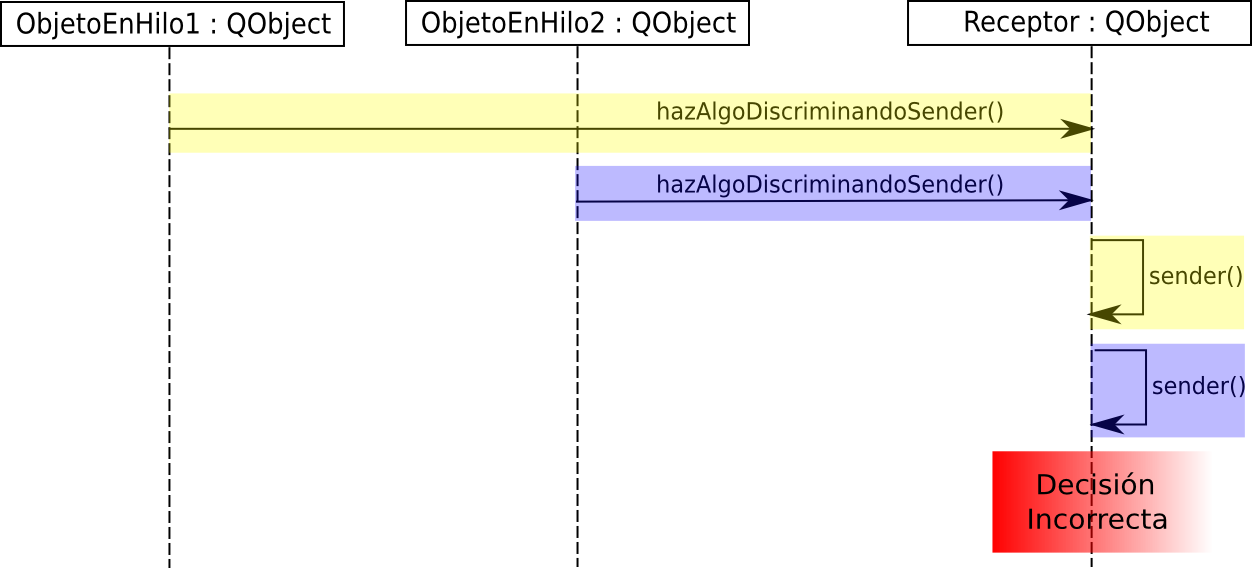
\includegraphics[scale=0.29]{diagSecuenciaSender.png}
    \medskip
    \begin{itemize}
        \item QObject::sender() no es compatible con el uso de hilos
        \begin{itemize}
            \item La emisión de una señal modifica el estado del receptor
        \end{itemize}
    \end{itemize}
\end{frame}

\begin{frame}[fragile]{QObject::sender() (2 de 2)}
    \framesubtitle{La solución - Multislots}
    \begin{itemize}
        \item Toman como primer parámetro quién ha emitido la señal
    \end{itemize}
\begin{lstlisting}[language=C++]
    static void receiver(Object *sender, int a, bool b)
    {
        // Codigo
    }
    ...
    class MiObjeto
        : public Object
    {
    public:
        ...
        IDEAL_SIGNAL(algoQueDecir, int, bool);
        ...
    }
    ...
    Object::connectStaticMulti(objeto->algoQueDecir, receiver);
\end{lstlisting}
\end{frame}

\begin{frame}[fragile]{Núcleo}
    \begin{itemize}
        \item Múltiples tipos de conexiones
        \begin{itemize}
            \item Señal $\rightarrow$ Slot
            \item Señal $\rightarrow$ Slot sincronizado
            \item Señal $\rightarrow$ Multi slot
            \item Señal $\rightarrow$ Multi slot sincronizado
            \item Señal $\rightarrow$ Slot estático / función
            \item Señal $\rightarrow$ Slot estático / función sincronizado
            \item Señal $\rightarrow$ Señal
        \end{itemize}
        \medskip
        \item Thread-safe
        \medskip
        \item Elementos básicos extensibles (Módulos)
        \begin{itemize}
            \item P.ej: obtención de información de ficheros
        \end{itemize}
\begin{lstlisting}[language=C++]
    File f1("file:///home/usuario/fichero.txt");
    File f2("ftp://ftp.servidor.com/fichero.txt");
    File f3("ssh://servidor.com/fichero.txt");
\end{lstlisting}
    \end{itemize}
\end{frame}

\begin{frame}{Interfaz Gráfica}
    \begin{itemize}
        \item Sencilla
        \medskip
        \item Potente
        \medskip
        \item Evitar código propenso a errores
        \begin{itemize}
            \item Evento $\rightarrow$ Nuevo thread
            \item Interfaz gráfica no bloqueable
        \end{itemize}
        \medskip
        \item Estilo
        \begin{itemize}
            \item Módulos
        \end{itemize}
        \medskip
        \item Cairo
        \begin{itemize}
            \item libX11
            \item libXrender
        \end{itemize}
    \end{itemize}
\end{frame}

\begin{frame}{Otras mejoras...}
    \begin{itemize}
        \item La interfaz gráfica no se bloquea fácilmente
        \item Extensiones
        \begin{itemize}
            \item Distintos protocolos soportados
            \item Distintos backends de dibujado
º           \item Extensible
        \end{itemize}
    \end{itemize}
\end{frame}

\frame{
  \frametitle{}
  \vspace{1.5cm}
  {\huge \alert{\textbf{Gracias.}} ¿Preguntas?}

  \vspace{3.5cm}
  \begin{flushright}
    Rafael Fernández López

    \structure{\footnotesize{ereslibre@kde.org}}
  \end{flushright}
}

\end{document}
